\documentclass[12pt,a4paper]{article}
\usepackage[utf8]{inputenc}
\usepackage[french]{babel}
\usepackage[T1]{fontenc}
\usepackage{amsmath}
\usepackage{amsfonts}
\usepackage{amssymb}
\usepackage{graphicx}
\title{Projet Méta-heuristique (MPRO) : Couverture connexe minimum dans les réseaux des capteurs}
\author{Groleaz Lucas \\ Houdayer Antoine}

\begin{document}
\maketitle
\tableofcontents
\part{Sujet}
\section{Modélisation}
Dans tous le problème, on recherche à placer des capteurs sur une grille de façon optimale. Autrement dit, on peut placer des capteur sur les point à coordonnées entières qui sont à l'intérieur d'une zone prédéfinie. Dans toute la suite on travaillera sur des grilles carrées, pour alléger les notations. On notera $n$ la dimension de la grille. Ainsi chaque sommet $v$ de la grille est un élément de $V=[\![1,n]\!]\times [\![1,n]\!]$. On notera $S\subset V$ l'ensemble des somment sur lesquels on a choisi de placer un capteur. 

Chaque capteur est doté d'un rayon de captation $R_{capt}$, et d'un rayon de communication $R_{comm}\geq R_{capt}$.  On souhaite utiliser un minimum de capteurs tout en respectant deux contraintes.
\begin{itemize}
\item Contrainte de connexité : La grille est doté d'un puits, point de coordonnées $(1;1)$. Un capteur peut communiquer avec tout capteur ou avec le puits, à condition qu'il soit séparé de ce dernier d'une distance inférieure ou égale à $R_{comm}$. Tout capteur doit pouvoir communiquer avec le puits, soit directement, soit par l'intermédiaire d'autres capteurs. 

\item Contrainte de couverture : Tout sommet de la grille, excepté le puits, doit être à une distance inférieure ou égal à $R_{capt}$ du capteur le plus proche.

\end{itemize}
\begin{figure}[!h]
\center
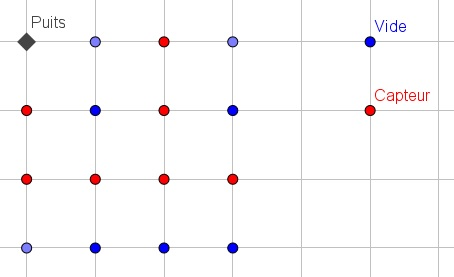
\includegraphics[scale=1]{Images/4_1_1_realisable.jpg}
\caption{Exemple de solution réalisable pour $n=4$, $R_{capt}=R_{comm}=1$, ici $|S|=7$}
\end{figure}
N.B: Il n'est pas interdit de couvrir le puits (ce qui est même inévitable si $R_{capt}=R_{comm}$), ou d'y placer un capteur, mais l'expérience montre qu'il n'est jamais intéressant de placer un capteur dans un coin de la grille. 
\section{Reformulation}
Nous avons adopté une reformulation du problème à base de graphes, un pour chaque contraintes. On note $p=(1;1)$, le puits. 
Pour une solution $S$ donnée, non nécessairement réalisable, on défini les ensembles d'arêtes $E_{capt}(S)$, l'en semble des liens de captations, et $E_{comm}(S)$ l'ensemble des liens de communication,  formellement.
\[E_{capt}(S)=\{\{v_1,v_2\}|v_1\in V\setminus p,\,v_2\in S\setminus v_1,\, \Delta(v_1,v_2)\leq R_{capt}\}\] 
\[E_{comm}(S)=\{\{v_1,v_2\}|v_1,\,v_2\in S\cup \{p\},\ v_1\neq v_2,\,\Delta(v_1,v_2)\leq R_{comm}\}\] 
On peut alors construire les graphes correspondants:
\[G_{capt}(S)=(V\setminus p,E_{capt}(S))\]
\[G_{comm}(S)=(S\cup p,E_{comm}(S))\]
Ci-dessous, une illustration dans le cas $n=4$, $R_{capt}=1$, $R_{comm}=2$. On a laissé tous les sommet de $S$ sur le schéma pour plus de lisibilité.
\begin{figure}[!h]
\center
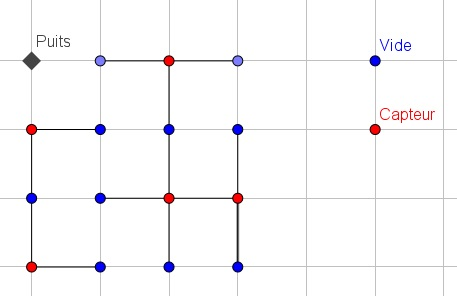
\includegraphics[scale=1]{Images/4_1_2_captgraph.jpg}
\caption{Graphe de captation $G_{capt}(S)$}
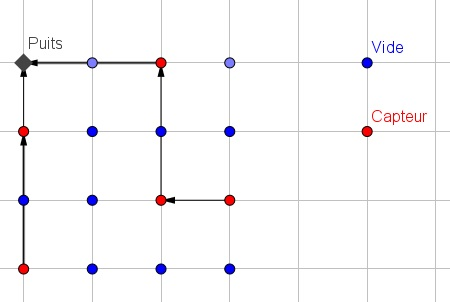
\includegraphics[scale=1]{Images/4_1_2_commgraph.jpg}
\caption{Graphe de communication $G_{comm}(S)$}
\end{figure}
\\N.B. : Sur le graphe de $G_{comm}$, on a représenté les arrêtes par des flèches, pour illustrer la notion de puits. Cependant, le graphe n'est pas intrinsèquement orienté, et il pourrait tout à fait présenter des cycles.

Le problème peut alors se reformuler de la façon suivante :
\begin{itemize}
\item Minimiser $|S|$.
\item Contrainte de connexité : $G_{comm}(S)$ est connexe.
\item Contrainte de couverture : $S$ est une couverture par les sommets de $G_{capt}(V\setminus p)$, ou dit d'une autre façon $G_{capt}(S)$ n'a pas de sommet isolé.
\end{itemize}
\section{Détails d'implémentation}
Nous avons choisi d'utiliser le langage $C++$ pour tenter d'implémenter une méthode de résolution approchée du problème. Nous avons taché d'utiliser une implémentation du problème alliant simplicité d'utilisation et efficacité. Pour cela, nous utilisons un codage double des solutions:

Pour garder en mémoire quels sont les sommet sur lequels un capteur est placé, le sommets captés, et les capteurs appartenant à la composant connexe du puits dans $G_{comm}(S)$, nous utilisons trois tableau de bits de type bitset. Leurs principals avantages sont leur faible occupation de mémoire, mais surtout la possibilité de les manipuler grâce à des opérations binaires. En contrepartie, leur taille doit être fixées à la compilation. Nous les avons déclarés de taille $2500$, pour traiter des grilles ayant moins de $2500$ sommets. Nous aurions du utiliser des vector<bool> pour pouvoir traiter des problème de taille arbitraire, mais en perdant la possibilité de faire des opérations binaires.

Nous gardons également en mémoire en permanence, les graphes $G_{comm}(S)$ et $G_{capt}(S)$, encodés comme étant pour chaque sommet, une liste de ses voisins dans le graphe, c'est-à-dire comme un tableau de listes de sommets. Pour être tout à fait rigoureux, plutôt que la structure "list" de la bibliothèque standard, nous avons créé une structure nommée GreedyList constitué d'un tableau pré-alloué associé à un compteur d'éléments. Ainsi, on évite les coûts de désallocation et allocation, principalement lors de la copie d'objets, gagnant un temps non négligeable. Ces graphes sont tout à fait  adaptés à la structure du problème et permettent d'être performant lors du calcul d'un nouvel état obtenu par suppression ou ajout d'un capteur. Il suffit pour cela de précalculer les deux graphes suivants : \[G_{capt}=G_{capt}(V\setminus p)\] le graphe de tous les liens de captation possibles, et \[G_{comm}=G_{comm}(V)\] le graphe de tous les liens de communication possibles. Un gros avantage de cette méthode est que l'on s'affranchit en partie de la définition initiale du problème. Pour peu que l'on puisse calculer les graphes $G_{comm}$ et $G_{capt}$, on peut facilement adapter le programme pour travailler sur des grilles (finies) de forme arbitraire, une disposition des points arbitraire, des calculs de distance différents, comme une portée différente suivant la position du capteur etc...

D'un point de vue plus pratique, sont codées les fonctions d'ajout et de suppression de capteur, qui gèrent l'utilisation et l'intégrité des objets mentionnés ci-dessus. On est alors libre d'utiliser ces fonctions et les dits objets pour travailler sur le problème. Notons que la fonction de suppression de capteur est relativement gourmande en calcul, puisqu'elle effectue un parcours en profondeur du graphe $G_{comm}(S)$ pour déterminer quelle est la nouvelle composante connexe du puits.



Nous avons alors essayé deux approches du problème très différentes.

N.B. il est assez pénible en pratique de placer un capteur sur le puits, nous ne le faisons jamais, comme ce n'est pas intéressant, on considérera éventuellement cela comme une possibilité dans les parties théoriques.
\part{Approche par chaînes de destruction}
Dans toute cette partie, on illustrera les méthodes présentées sur l'instance $(P)$ du problème : $n=4$, $R_{capt}=R_{comm}=1$.
\section{Heuristique}
\subsection {Heuristique déterministe}
Dans cette approche, on construit tout simplement une solution $S$ en positionnant des capteurs sur la totalité de la grille, pour avoir une solution réalisable. On tente alors de retirer les capteurs un à un lorsque c'est possible sans compromettre la réalisabilité de la solution. Il s'agit pour cette raison d'une heuristique destructrice.
Illustrons la méthode sur $(P)$ : 
\begin{figure}[!h]
\center
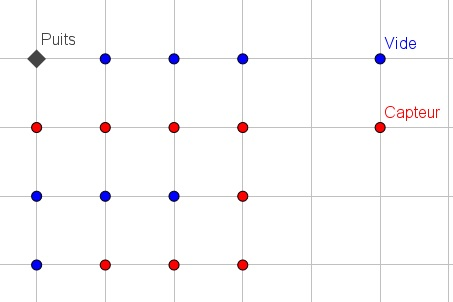
\includegraphics[scale=1]{Images/4_1_1_naif.jpg}
\caption{Résultat de l'heuristique de destruction sur $(P)$}
\end{figure}

Procédons dans l'ordre, ligne par ligne :  on peut enlever la première ligne sans problème, cependant, on doit alors conserver $(2;1)$ pour ne pas déconnecter le reste des capteurs. On doit également garder le reste de la seconde ligne pour continuer à capter la première. On peut alors retirer la troisième ligne, à l'exception de $(3;4)$ qui est alors nécessaire pour connecter la dernière ligne. On peut ensuite enlever $(4,1)$. On constate qu'on est alors obligés de garder le reste de la dernière ligne.

Si l'on note les sommet par leur indice $k=n*(i-1)+(j-1)$ plutôt que part leur coordonnées $(i;j)$, pour plus de concision, on obtient
\[S=\{4,5,6,7,11,13,14,15\}\]

A première vue, cette heuristique présente de quelques défauts, et assez peu de qualités. Tout d'abord cette heuristique est chronophage : on essaye de retirer un a un les capteurs (initialement au nombre de $n^2$), ce qui implique d'effectuer un parcours en profondeur des sommets restants pour vérifier la connexité. Le coût de construction d'une telle solution est donc de $O(n^4)$. Deuxièmement, la structure induite par une telle construction est peu désirable en pratique, sauf justement dans le cas $R_{capt}=R_{comm}=1$, on obtient en général des solutions de qualité médiocre. Elle a toutefois l'avantage d'être implémentée en seulement quatre lignes de code. Elle a également l'avantage de garantir que la solution obtenue est réalisable. 

Attention : contrairement à ce que la construction pourrait laisser penser, il est rare, mais possible d'obtenir une solution dans laquelle il est toujours possible d'enlever un capteur (on appellera solution dégénérée une telle solution). En effet, il est possible qu'un capteur soit nécessaire pour conserver la connexité, mais qu'il devienne facultatif après avoir enlevé un de ses voisin. Cela est toutefois rare et marginal, c'est pourquoi cette heuristique produit tout de même des solutions "acceptables".
\subsection{Heuristique aléatoire} 
On peut apporter à cette heuristique une très simple,visant à briser la structure induite par la méthode. Pour cela, il suffit de remarquer que la solution obtenue est  dépendante de l'ordre dans lequel on a essayé de retirer les sommet (ligne par ligne dans l'exemple). On choisit alors au hasard un ordre dans lequel on va retirer les capteurs, c'est-à-dire une permutation des sommets. Par exemple si on tire au hasard la permutation suivante : \[0,10,11,12,13,5,8,15,9,6,4,3,14,1,2,7\] on obtiendra le résultat représenté sur la figure ci-dessous:
\begin{figure}[!h]
\center
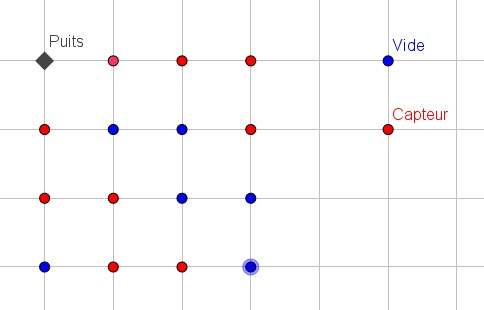
\includegraphics[scale=1]{Images/4_1_1_random.jpg}
\caption{Résultat pour une permutation au hasard}
\end{figure}

Bien sûr, cela ne garantie pas l'obtention d'une meilleur solution mais donne effectivement des solution meilleures en moyenne que celles de l'heuristique déterministe, pour une instance quelconque. En annexe est fourni un jeu de résultats obtenus sur les instances de test.

Dans toute la suite de la partie, on dénote par $S^b$ le vecteur binaire associé à $S$, de sorte que $S^b_{n(i-1)+(j-1)}=1$ si et seulement un capteur est présent en $(i;j)$. Les indice vont donc de $0$ pour le  puits à $n^2-1$ pour le sommet inférieur droit, $S^b$ est de longueur $n^2$. Ici, 
\[S^b=[0,1,1,1,1,0,0,1,1,1,0,0,0,1,1,0]\]

\section{Les chaînes de destruction}
\subsection{Définition}
Le procédé décrit ci-dessus à été conçu avec le problème présent en tête, mais on pourrait tout à fait l'appliquer à n'importe quel problème d'optimisation binaire dans lequel on veut maximiser le nombre de bits à $1$ dans le vecteur solution. On pourrait aussi adapter le procédé pour la minimisation en partant d'un vecteur nul, et en mettant progressivement des bits à $1$. Par exemple, l'algorithme glouton du problème de sac à dos classique consiste en fait à appliquer cette méthode en utilisant une permutation obtenue grâce à un heuristique d'utilité.

Cela permet de supposer qu'améliorer l'heuristique consisterait à trouver une "bonne" permutation. 

Nous appellerons chaîne de destruction, et on notera $l$, la permutation utilisée, c'est-à-dire l'ordre dans lequel on a tenté de retirer les capteurs (i.e. de mettre les bits à 0 dans $S^b$). On notera $S(l)$ la solution engendrée par $l$.
\subsection{Propriétés}
\subsubsection{Chaîne de destruction d'une solution non dégénérée}
\paragraph{Définitions et énoncé} 
Soit $S$ une solution non dégénérée. On rappelle que cela signifie qu'il est impossible de retirer un capteur (i.e. de mettre un bit à $0$ dans $S^b$) sans violer une contrainte. On définit alors $l^c$ comme étant la liste dans un ordre arbitraire des indices $k$ pour lesquels $S^b_k=1$, c'est-à-dire la liste des position sur lesquelles il y a un capteur. De même on définit $l^e$ comme étant la liste dans un ordre arbitraire des indices $k$ pour lesquels $S^b_k=0$. On note $l^e+l^c$ la concaténation de ces deux listes (avec $l^e$ en premier). Par définition $l^e+l^c$ contient une et une seule fois tous les entier compris entre $0$ et $n^2-1$, et est donc bien une chaîne de destruction. On observe alors ,dans notre problème mais pas nécessairement dans un cas plus large, la propriété suivante
\[S=S(l^e+l^c)\]
\paragraph{Démonstration}

Soit $S$ une solution réalisable quelconque. Montrons qu'en ajoutant un capteur à $S$ on obtient toujours une solution réalisable (mais nécessairement dégénérée il va de soi). Trivialement, la contrainte de couverture est toujours vérifiée, en ajoutant un sommet à une couverture par les sommets de $G_{capt}(V\setminus p)$ on obtient toujours une couverture valide car le graphe $G_{capt}(V\setminus p)$ n'est pas fonction de $S$. Le graphe $S$ avant ajout du capteur vérifiant la propriété de couverture, on ajoute le capteur à endroit qui était couvert ( ou sur le puits, auquel cas il n'y a pas de problème puisque le puits est de base dans le graphe de connexité), c'est-à-dire à distance inférieure ou égale à $R_{capt}$ d'un autre capteur. Or, $R_{comm}\geq R_{capt}$, le nouveau capteur pourra donc se connecter à un ancien, le nouveau graphe $G_{comm}(S)$ sera bien toujours connexe.


Ainsi, on a démontré qu'on pouvait passer de $S$ à une grille remplie en passant par des solutions réalisable en ajoutant les capteurs dans un ordre arbitraire.

Il est alors vrai qu'en retirant un à un les élément de $l^e$ dans un ordre arbitraire à une grille remplie, on effectue le chemin inverse.

Enfin par définition d'une solution non dégénérée il sera impossible de retirer les capteurs de $l^c$ quelle que soit l'ordre.

Remarque : Je remarquais précédemment que notre implémentation permettait de traiter des variantes avec d'autres définitions de distance. On voit ici que cette propriété (et les méthodes qui en découlent) n'est vraie que si à chaque possible lien de captation correspond un lien de communication, puits exclu, c'est à dire puits exclu $G_{capt}\subset G_{comm}$. En particulier, il serait impossible de travailler avec cette heuristique si on avait $R_{comm}<R_{capt}$.

On a donc démontré que pour chaque solution non dégénérée (et a fortiori toute solution optimale) on pouvait construire facilement une chaîne de destruction qui la génère, et donc qu'il en existe une. On peut donc en toute légitimité encoder un solution non dégénérée (et donc a fortiori optimale) par une de ses chaînes de destruction. Moralement on démontre que les chaînes de destruction sont adaptés pour résoudre le problème que l'on se pose.  

On rappelle qu'il est malheureusement possible pour une chaîne de destruction d'engendrer une solution dégénérée, ce qui est quelque peu une épine théorique, mais jamais un problème en pratique.

\subsubsection{Chaînes équivalentes}
Lorsqu'on code une solution quelconque, pas forcément réalisable, avec son vecteur binaire, il découle immédiatement pour une grille de dimension $n$, il existe $2^{n^2}$ solutions possible. De plus, seulement une partie infime de ces solutions, parmi les solution réalisables seulement, et incluant les solution non dégénérées, peut être associée à une chaîne de destruction.

Or, une chaîne de destruction étant essentiellement une permutation, il existe $n^2!\gg 2^{n^2}$ chaînes de destruction. On en déduit qu'il existe nécessairement pour chaque chaîne de destruction un nombre colossal de chaînes de destruction équivalentes, c'est-à-dire engendrant la même solution.

En particulier, on vient de montrer que pour une solution S non dégénérée, on peut mélanger comme on souhaite $l_e$ et $l_c$, et obtenir par concaténation une chaîne de destruction équivalente.

On pourrait montrer que de façon plus générale, que pour une chaîne de destruction $l$, on peut mettre à la fin de la chaîne les indices des capteur que l'on a pas pu retirer, sans changer leur ordre relatif. On peut ensuite mélanger de façon interne le début de la chaîne constitué a des indice des capteurs qu'on a pu enlever. On peut aussi mélanger la fin de la chaîne de la même manière si la solution engendrée est non dégénérée.

D'un point de vue encodage d'une solution, on peut donc voir une chaîne de destruction comme une partition des sommets entre $S$ et $V\setminus S$ (il faut cependant appliquer la chaîne de destruction pour connaître la partition qu'elle encode).

\section{Voisinage induit}
\subsection{Définition et propriétés}
Lorsque qu'on cherche une structure de voisinage, on chercher un façon qui fait sens de modifier légèrement le vecteur qui encode la solution. Par exemple dans le problème du sac à dos, on peut essayer d'ajouter un objet dans le sac, quitte à appliquer après une heuristique de réparation. Dans notre problème on souhaiterait par exemple déplacer légèrement un capteur, ou en supprimer quelques uns. Il n'est cependant pas facile de faire une heuristique de réparation assez efficace pour avoir une meilleur solution après.

C'est là qu'est la force des chaînes de destruction : en appliquant une légère modification à une chaîne de destruction et en l'appliquant, on obtient une solution S légèrement modifiée, réalisable et selon toute probabilité non dégénérée !  

Le voisinage utilisé par la suite est le suivant :
Soit $S$ une solution. On construit les suites $l^e$ et $l^c$, puis on les mélange aléatoirement. On choisit au hasard un élément de $l^c$, qu'on retire de $l^c$ pour le mettre au début de $l^e$. On appelle $l'^e$ et $l'^c$ les suites ainsi obtenues. On construit alors une nouvelle solution $S'$ à partir de $l'=l'^e+l'^c$.
En faisant cela, on choisi en fait au hasard un capteur et on met son indice au début de la chaîne de destruction, on va donc faire en sorte  de ne pas mettre de capteur à cet endroit. La nouvelle chaîne $l'$ ne peut donc pas générer la solution que $S'$.

Remarques:

Sans que ce soit gênant, on peut noter que $S$ n'est pas nécessairement dans le voisinage de $S'$.

Par ailleurs, toujours sans que ce soit gênant,si $S$ est dégénérée, il se peut que $S(l)$ avec $l=l^e+l^c$ ne soit pas "proche" de $S$. Il va alors de soit que $S'$ n'est pas nécessairement proche de $S$.

Dernière remarque, pourquoi, sous l'hypothèse que $S$ ne soit pas dégénérée, $S'$ est-elle proche de $S$? Sans avoir une preuve de ce que j'avance ici, on constate et c'est logique que plus un capteur est proche du début de la chaîne de destruction, plus la probabilité qu'on puisse l'enlever est élevée. Puisque on a juste déplacé un seul élément(si $S$ est non dégénérée, le mélange est toujours équivalent), les élément du début de $l$ sont au début de $l'$, et vice-versa. Les solutions engendrés sont donc toujours proches, d'expérience. Je pense qu'il est possible dans de rare cas que $S'$ soit assez différente de $S$, mais je ne l'ai jamais observé.
\subsection{Exemple}
Soit la solution non dégénérée obtenue avec l'heuristique déterministe.
On rappelle qu'on avait alors
\[l=(0,1,2,3,4,5,6,7,8,9,10,11,12,13,14,15)\] 
\[S(l)=\{4,5,6,7,11,13,14,15\}\]
\begin{figure}[!h]
\center
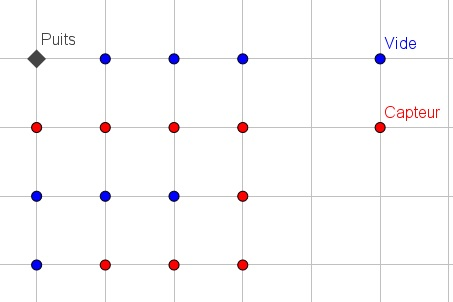
\includegraphics[scale=1]{Images/4_1_1_naif.jpg}
\caption{Résultat de l'heuristique de destruction sur $(P)$}
\end{figure}

On construit donc 
\[l^e=(0,1,2,3,8,9,10,12)\]
\[l^c=(4,5,6,7,11,13,14,15)\]
On mélange aléatoirement
\[l^e=(8,0,9,10,3,1,12,2)\]
\[l^c=(13,7,5,6,15,11,14,4)\]
On prend un sommet de $l^c$ qu'on met au début de $l^e$, par exemple $15$, on impose alors de ne pas mettre de capteur dans le coin inférieur droit.
\[l'^e=(15,8,0,9,10,3,1,12,2)\]
\[l'^c=(13,7,5,6,11,14,4,12)\]
On obtient alors 
\[l'=(15,8,0,9,10,3,1,12,2,13,7,5,6,11,14,4)\]
A première vue, il pourrait sembler que cette chaîne de destruction est très différente de la chaîne ordonnée, pourtant en appliquant la chaîne, on obtient
\[S'=\{4,5,6,7,10,13,14\}\]
Non seulement on est sur une solution très proche, mais elle utilise même un capteur en moins.
\begin{figure}[!h]
\center
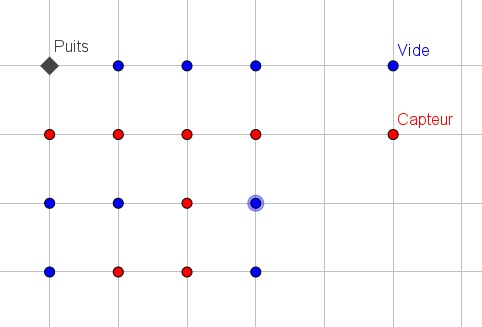
\includegraphics[scale=1]{Images/4_1_1_neigh.jpg}
\caption{Voisinage de la solution déterministe}
\end{figure}

Remarques : La taille du voisinage est est démesurée, il est déconseillé d'appliquer des technique de parcours méthodique telles que la recherche de voisinages améliorants, ou la recherche avec tabous. Dans la section suivante, on l'utilise dans l'algorithme du recuit simulé.
\end{document}